\section{Introduction}
\label{sec:intoduction}
Large language model (LLM) pre-training has been largely democratized and open-sourced, allowing various academic labs, and industries to pre-train custom LLMs. 
Yet, a key differentiator between these models is the composition and size of the data used to train them. 
Data curation strategies are required to filter out scrapes of the web that are unstructured and/or poorly phrased~\citep{eisenstein-2013-bad}.
While some of these strategies have been made public~\citep{brown2020language,wenzek-etal-2020-ccnet,penedo2023refinedweb}, most state-of-the-art data curation techniques are unknown to the research community, and only anecdotal evidence remains. Research on data curation requires multiple rounds of re-training, making it an expensive endeavour to document techniques that lead to practical improvements.
On the other hand, scaling laws for language models (such as Chinchilla scaling laws~\citep{hoffmann2022training}) show that with increasing model sizes, we should also increase both the training compute and data size linearly.  This is infeasible because (a) high-quality data is limited \citep{villalobos2022will}, and repeating for even a small number of epochs (4 or more) results in diminishing returns or overfitting \citep{muennighoff2023scaling,touvron2023llama,xue2023repeat}; and (b) pre-training for such long durations is prohibitively expensive. 

Meanwhile, the use of synthetic data has gained prominence in the paradigm of aligning pre-trained LLMs via instruction fine-tuning, RLHF~\citep{ouyang2022training}, and instruction backtranslation \citep{li2023self}. 
Recently, in the context of pre-training, synthetic data was used to generate datasets such as Tiny Stories~\citep{eldan2023tinystories}
and Textbook quality synthetic data~\citep{gunasekar2023textbooks,li2023textbooks}.  These were used to train smaller language models (like the Phi model family) that were as performant as larger language models on certain tasks.  
However, their data generation process stays largely opaque, and prohibitively expensive, requiring prompting a GPT-3.5 model for generating billions of tokens. Additionally, such data generation can create a large ``knowledge bias'' by specifically generating data pertaining to tasks that we want to perform well on. While synthetic data has shown promise, it is unclear if this is because of the higher quality nature of synthetic data, or because of strategic topic selection~\citep{maini_phi_1_5}.
\begin{figure}[t]
    \centering
       \begin{subfigure}{0.32\textwidth}
        \centering
        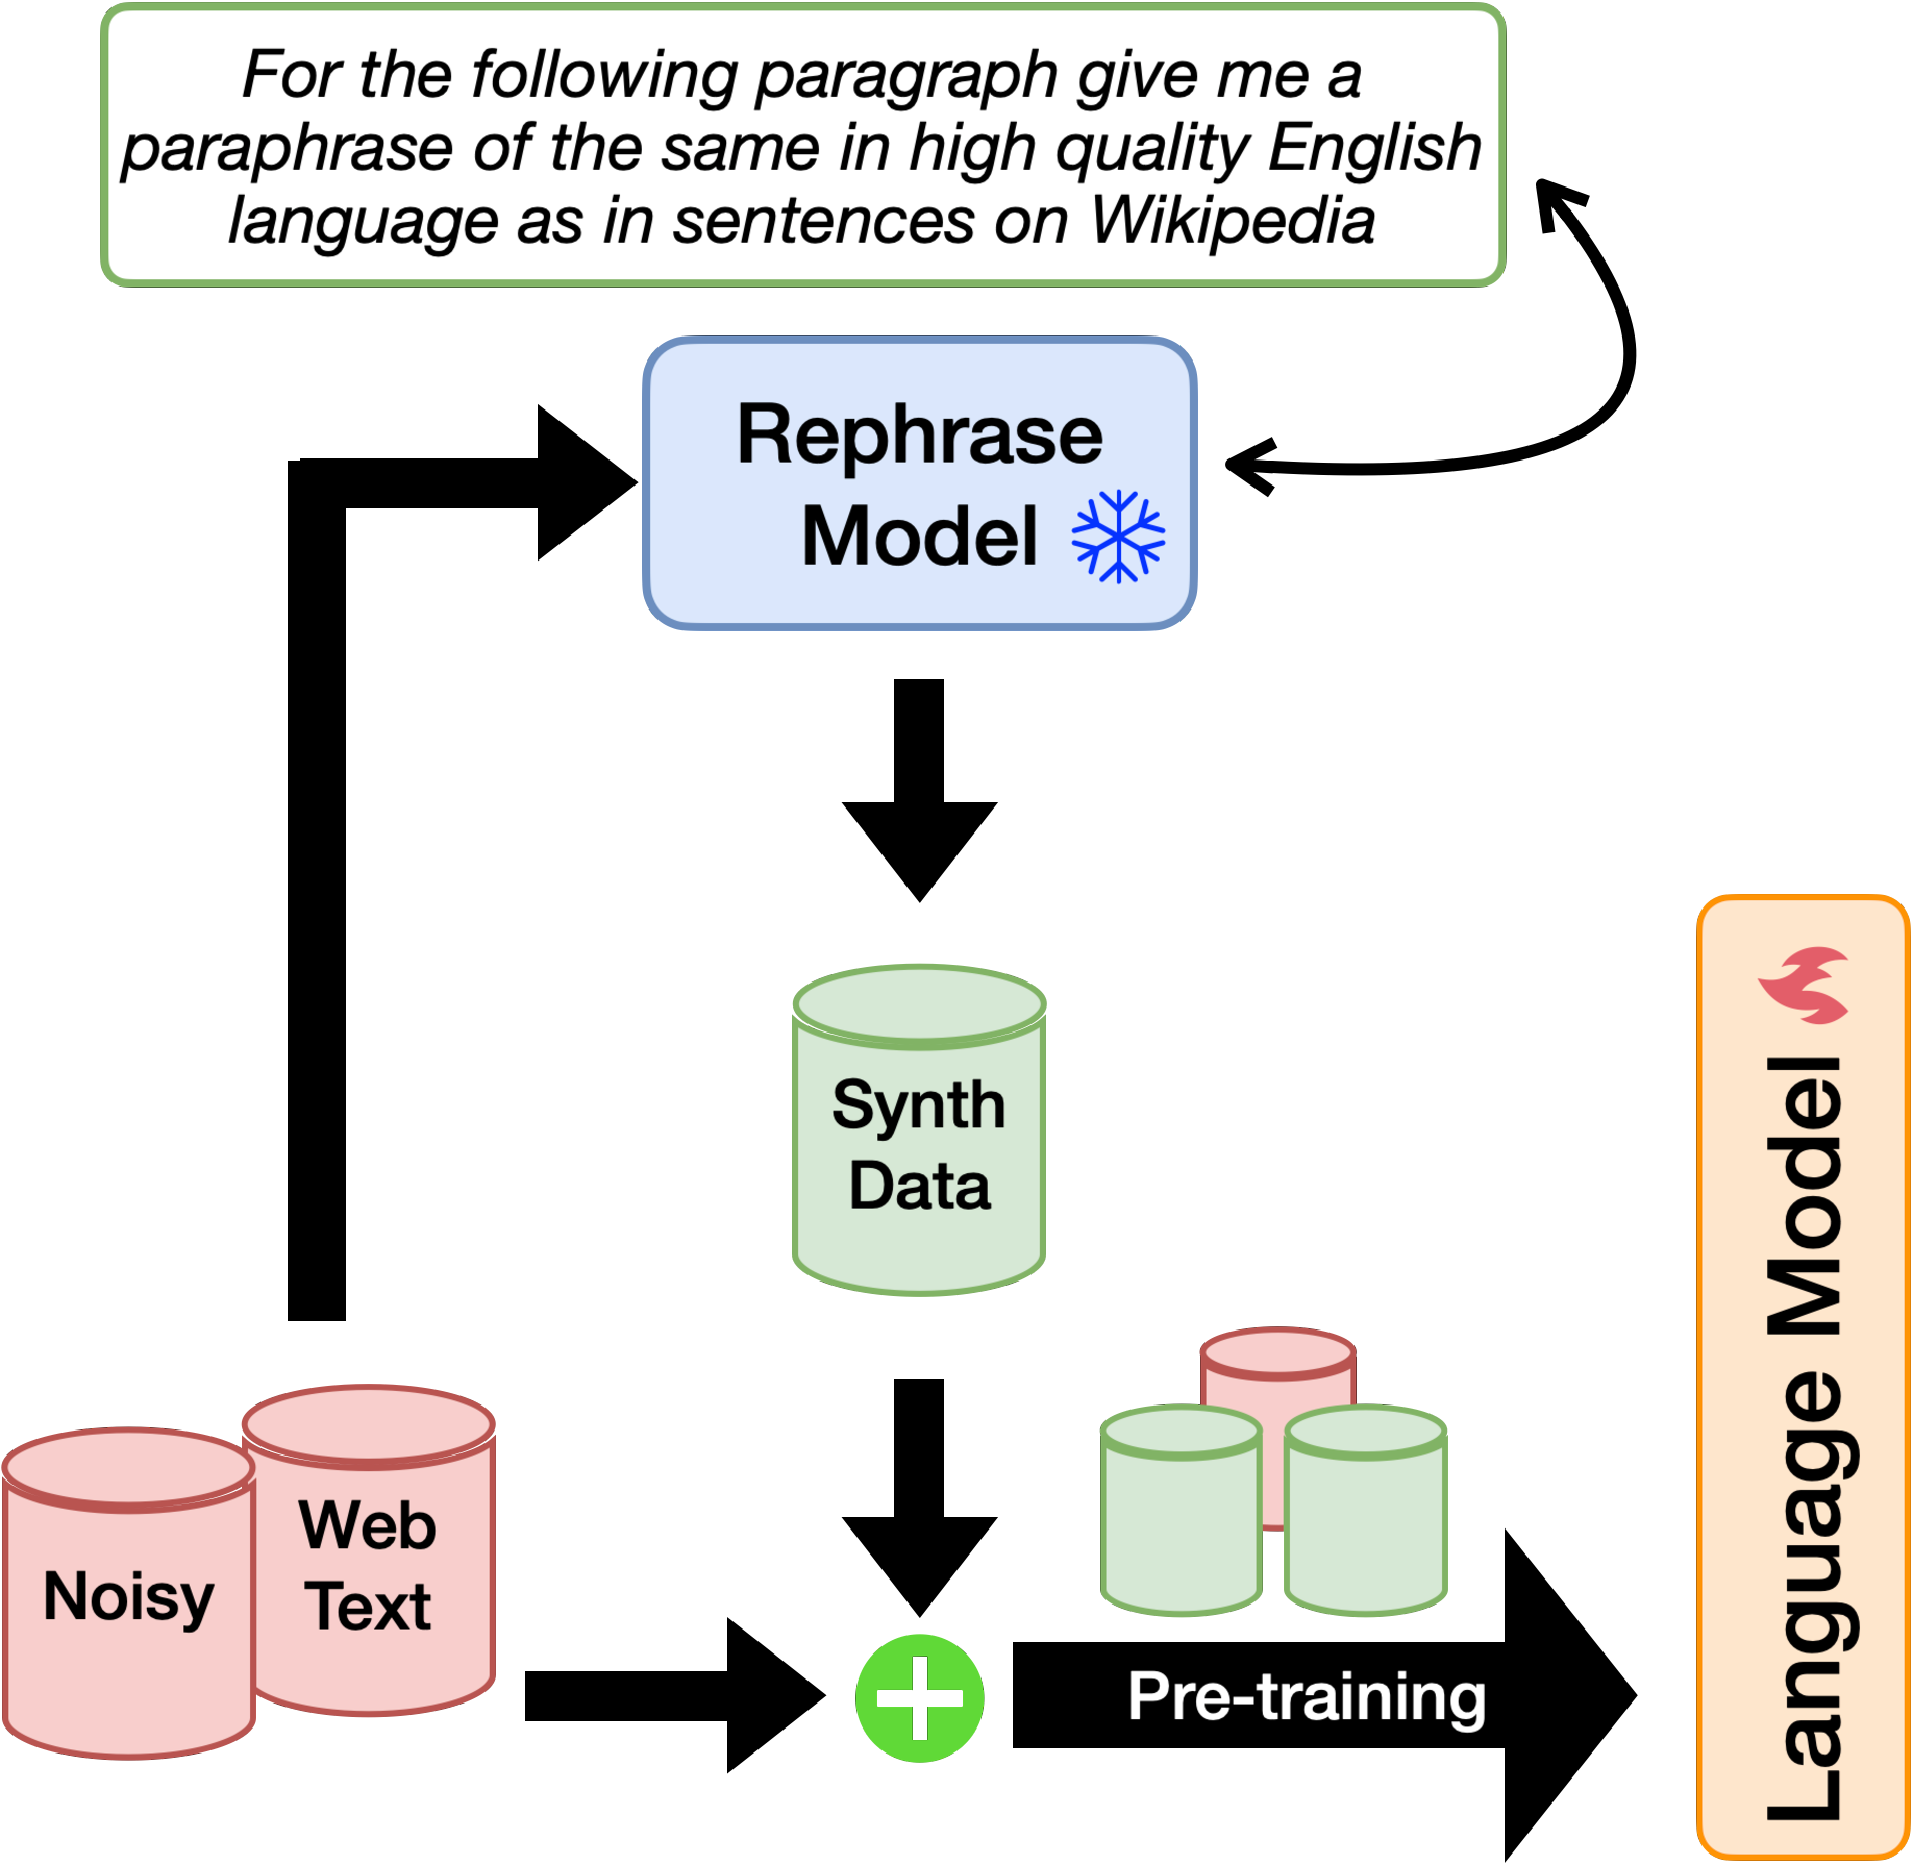
\includegraphics[width=\textwidth]{figures/method.pdf}
        \caption{}
        \label{fig:method}
        \vspace{2mm}
    \end{subfigure}
    \hfill
    \begin{subfigure}{0.32\textwidth}
        \centering
        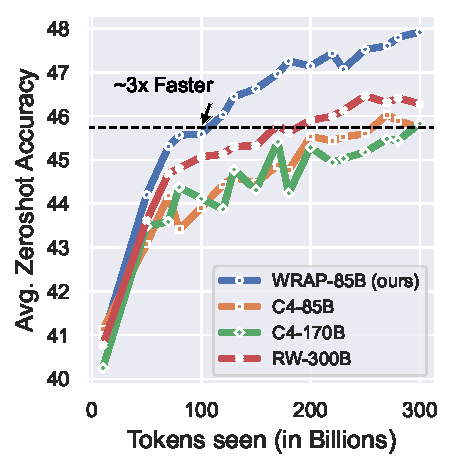
\includegraphics[width=\textwidth]{figures/qa_scaling_plot.pdf}
        \caption{}
        \label{fig:upper_right_image}
    \end{subfigure}
    \hfill
    \begin{subfigure}{0.32\textwidth}
        \centering
        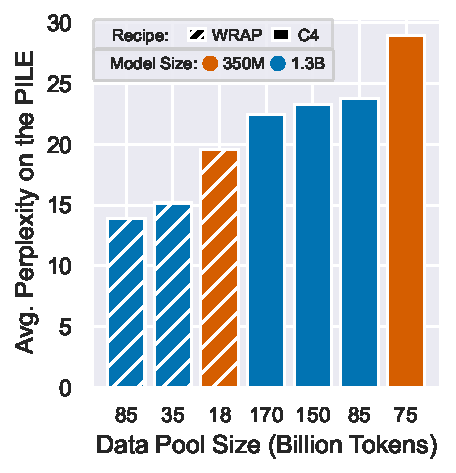
\includegraphics[width=\textwidth]{figures/pile_scaling_curves_perplexity.pdf}
        \caption{}
        \label{fig:lower_right_image}
    \end{subfigure}

    \caption{(a) \ours~Recipe: We prompt an off-the-shelf instruction-tuned model to rephrase articles on the web, and pre-train an LLM on a mixture of real and synthetic data. ~(b) Zero-shot performance of GPT 1.3B models trained on combinations of C4 and synthetic variations. Each step corresponds to a batch of 1M samples. (c) Weighted average perplexity over 21 sub-domains of the Pile for varying model sizes and amount of pre-training data.}
    \label{fig:common_caption}
\end{figure}



In this work, we propose \textbf{W}eb \textbf{R}ephrase \textbf{A}ugmented \text{P}re-training~(\ours)---that attempts to bridge
three important challenges stemming from the ambiguity around data curation---
(i) what data should you pre-train on?
(ii) how can you pre-train with limited data?
(iii) how can you pre-train computationally efficiently?
In particular, we show that re-phrasing documents on the web using an off-the-shelf medium size LLM allows models to learn much more efficiently than learning from raw text on the web, and 
accounts for 
performance gains on out of distribution datasets that \emph{can not} be offset with additional web data. Our proposed method involves using a pre-trained off-the-shelf LLM to re-phrase documents from a web corpus into different styles.  An overview of our approach is shown in Figure~\ref{fig:method}.




In our work, we tackle two important challenges faced during synthetic data curation in the works of~\citet{gunasekar2023textbooks}---generation cost, and data bias---by rephrasing articles on the web. (i) \ours~allows for using an open source, and much smaller LLM (1.8B/7B v/s GPT3.5) to rephrase unstructured and poorly phrased documents in different styles, since it does not rely on the LLM as a knowledge bank. (ii) Thanks to the information maintaining nature of rephrasing, we are able to leverage the natural diversity of the web, rather than relying on an LLM for information which may be prone to factual errors, and/or data biases. Our work shows that the ``style'' alone can result in large gains in downstream performance.

Using \ours~on the C4, we evaluate model performance on 13 different zero-shot tasks, and 21 different language modeling domains of the Pile,  and find that pre-training LLMs with synthetic data allows us to train equivalent models with 5x lesser data, or 3x lesser compute. In fact, our synthetic data trained models, also outperform the recent TinyLLama models that were trained for 3 trillion tokens (10x data and compute) across several zero-shot Q/A tasks. 
We further observe 
a reduction in perplexity by $\sim50\%$ on the Pile,
and note that our 350M parameter model trained on combinations of real and synthetic rephrases on just $15\%$ of the entire C4 corpus,  outperforms pre-training a 1.3B parameter on the entire C4.
Finally, we conduct an analysis on the 
potential of data leakage, 
properties of synthetic data styles, and how to combine synthetic data for improving  \ours~based LLM pre-training.
